\chapter{Towards Model-based Run-time State Migration}
\label{ch:requirements}

\section{Requirements Analysis}

A requirement analysis shall be applied to identify what an approach for run-time state migration has to offer. This approach shall enable modeling run-time states, in general, to know which migratable run-time states are involved in the application's scope. Also, we need to find at least two existing applications which are suitable to apply this approach.

\subsection{R1 Applicable on Existing Applications}
This approach shall allow enabling run-time state migration on new and existing same-purpose applications. Developers should be able to use this approach on applications, even if they are not part of the applications' developers team. Thereby, it enables the support of a vast number of existing applications.


\subsection{R2 Platform-independent State Specification}
It shall be possible to model which and when parts of existing applications can be migrated. Also, it shall be possible to model these states in a platform-independent manner.

\subsection{R3 Model Repository}
Developers have to adapt the run-time state migration approach to existing applications. Thereby, they have to find an existing state specification or define their own. So, it shall be possible to have a central place to store models that are state specifications which developers can search for common models or upload models they defined.

\subsection{R4 Device Management}
It must be possible to find, retrieve and select devices offering the same states and migrate them. Also, the device discovery shall be possible in a way that the approach can express if an application knows another application has the same state on the same network.



\section{Requirements for a DSL}
Based on \textbf{R2 Platform-independent State Specification}, we chose to develop a DSL to model the run-time states by specifications. 
We have identified the most common structure a state has and defined them as requirements for a DSL to specify a state as follows.


\subsection{D1 State Specification}
The DSL shall be able to provide the specification of a state by defining a model. State whose are following these specifications can be migrated between applications explicitly or implicitly. Also, state specification shall provide a way to define what part of a run-time state is required and what part is optional.

\subsection{D2 Finding Same Model}
To find common models between applications, the DSL must allow specifying a way for finding the same model. These specifications can be a unique model name and model version.

\subsection{D3 Validating}    
In case of improving the DSL for long-time support, the DSL must have a version to allow validating the state specification. So, it can be possible to know the state specification using which version of the DSL.



\section{Same-purpose Applications Analysis}
The following analysis is to determine what pairs of application states exist and what needs to be modeled.
These applications are from different platforms, and they are interactive applications for end-users and have sufficient complexity (e.g., applications should not have only one single state).


\subsection{State Analysis of Applications}
In this section, we compared four pairs of applications to determine which states are common between applications. Also, the type of the states is categorized into three types which are run-time state (R), persistent state (P), and action (A). Furthermore, the Migratable column shows if the state can be a candidate for run-time state migration.

\subsubsection{States of E-mail Applications}

Table \ref{tab:states_of_email_applications} shows a list of available states of two open-source e-mail clients: Mailspring on macOS and K-9 Mail on Android. Some states are migratable like "Single E-mail" and "Search View". The "Single E-mail" state contains a view of a single e-mail in reading mode. In "Search View" the user can search and find an e-mail by typing in a query input box. The information of some states like "Compose a new E-email", "Forward an E-mail" and "Replay an E-mail" are almost similar, and they can be considered as one state for sending an e-mail.

\begin{table}[ht!]
\begin{tabular}{lll|ll}
State / E-mail client                   & Mailspring                & K-9 Mail                  & Type & Migratable                 \\ 
\hline
Welcome   Screen                        & \checkmark & \checkmark & P    &                            \\
Account Registration                    & \checkmark &                           & P    &                            \\
Account Login                           & \checkmark &                           & P    &                            \\
Add an e-mail service account           & \checkmark & \checkmark & P    &                            \\
Import   Settings                       &                           & \checkmark & P    &                            \\
Export Settings and Accounts            &                           & \checkmark & P    &                            \\
Settings                                & \checkmark & \checkmark & P    &                            \\
Sync New E-mails                        & \checkmark & \checkmark & P    &                            \\
Compose a   new E-email                 & \checkmark & \checkmark & R    & \checkmark  \\
Forward an E-mail                       & \checkmark &                           & R    & \checkmark  \\
Replay an   E-mail                      & \checkmark & \checkmark & R    & \checkmark  \\
Sending an E-mail                       & \checkmark & \checkmark & A    &                            \\
Trashing   an E-mail                    & \checkmark & \checkmark & A    &                            \\
E-mails list (Inbox, Sent, Draft, …)    & \checkmark & \checkmark & P    &                            \\
Single   E-mail                         & \checkmark & \checkmark & R    & \checkmark  \\
Show Original Version of E-mail         & \checkmark &                           & R    &                            \\
Search   View                           & \checkmark & \checkmark & R    & \checkmark  \\
Searching                               & \checkmark & \checkmark & A    &                            \\
Loading   E-mails                       & \checkmark & \checkmark & A    &                            \\
Loading Activity Data                   & \checkmark &                           & A    &                            \\
Activity   View                         & \checkmark &                           & P    &                            \\
Exporting Activity Data                 & \checkmark &                           & A    &                            \\
Sharing   Report of Activity Data       & \checkmark &                           & A    &                            \\
Marking Star/Spam/Read/Unread an E-mail & \checkmark & \checkmark & A    &                           
\end{tabular}
\caption{States of E-mail Applications}
\centering
\label{tab:states_of_email_applications}
\end{table} \FloatBarrier

\newpage
\subsubsection{States of Browsers}

Table \ref{tab:state_browsers} shows a list of available states of two browser applications: Firefox on macOS and Chrome on Android. The information in the current tab can be found in the "Current Tab" state. Also, searching is possible within the "Finding" state. Information of "Developer Console" and "Private/Incognito Mode" states is whether they are opened as a window or not.

Some states information are form official Chrome Page lifecycle API\footnote{\href{https://developers.google.com/web/updates/2018/07/page-lifecycle-api}{https://developers.google.com/web/updates/2018/07/page-lifecycle-api}} and Mozilla Web API\footnote{\href{https://developer.mozilla.org/en-US/docs/Web/API}{https://developer.mozilla.org/en-US/docs/Web/API}}. Also, For browsers there is a standard called W3C Page lifecycle API\footnote{\href{https://wicg.github.io/page-lifecycle/}{https://wicg.github.io/page-lifecycle/}}.


\begin{table}[ht!]
\begin{tabular}{lll|ll}
State / Browser                                       & Firefox           & Chrome          & Type & Migratable                 \\ 
\hline
Home page                                             & \checkmark & \checkmark & P    &                            \\
Single Tab (Preferences, Bookmarks, Performance,   …) & \checkmark & \checkmark & P    &                            \\
Extensions   Tab                                      & \checkmark &                           & P    &                            \\
Syncing                                               & \checkmark & \checkmark & A    &                            \\
Browsing                                              & \checkmark & \checkmark & A    &                            \\
Current Tab                                           & \checkmark & \checkmark & R    & \checkmark  \\
Developer   Console                                   & \checkmark & \checkmark & P    &                            \\
Signing in                                            & \checkmark & \checkmark & A    &                            \\
Finding   (in page)                                   & \checkmark & \checkmark & R    & \checkmark  \\
Printing                                              & \checkmark &                           & A    &                            \\
Downloading                                           & \checkmark & \checkmark & A    &                            \\
Sharing                                               &                           & \checkmark & A    &                            \\
Private/Incognito   Mode                              & \checkmark & \checkmark & R    & \checkmark  \\
Light mode                                            &                           & \checkmark & R    &                           
\end{tabular}
\caption{States of Browsers applications}
\label{tab:state_browsers}
\end{table} \FloatBarrier


\subsubsection{States of Video Player Applications}
Table \ref{tab:states_video_players} shows a list of available states of two video player applications which are IINA on macOS and VLC on Android. In these applications, all migratable states' information is the status of playing a video and can be considered almost identical. These states are "Pause", "Playing Video" and "Streaming". 

To support run-time state migration on video players, we needed to access the video file, considering the video's size is not the right choice. However, run-time state migration can be supported on video streaming applications with the same media.


\begin{table}[ht!]
\begin{tabular}{lll|ll}
State / Video Player                                  & IINA                      & VLC                       & Type & Migratable                 \\ 
\hline
Welcome   Screen                                      & \checkmark & \checkmark & P    &                            \\
Video player tips                                     &                           & \checkmark & P    &                            \\
Audio   player tips                                   &                           & \checkmark & P    &                            \\
Pause                                                 & \checkmark & \checkmark & R    & \checkmark  \\
Deleting                                              &                           & \checkmark & A    &                            \\
Browsing view                                         & \checkmark & \checkmark & R    &  \\
Loading   Directories                                 &                           & \checkmark & A    &                            \\
Single Page view (About, Settings, Audio,   Video, …) & \checkmark & \checkmark & P    &                            \\
Search   result                                       &                           & \checkmark & R    &  \\
Searching                                             &                           & \checkmark & A    &                            \\
Playing   video                                       & \checkmark & \checkmark & R    & \checkmark  \\
Playing audio                                         & \checkmark &                           & R    &                            \\
Showing   picture                                     & \checkmark &                           & R    &                            \\
Streaming                                             & \checkmark & \checkmark & R    & \checkmark  \\
Loading   local network devices                       &                           & \checkmark & A    &                           
\end{tabular}
\caption{States of Video player applications}
\label{tab:states_video_players}
\end{table} \FloatBarrier

\newpage
\subsubsection{States of Note Taking Applications}
Table \ref{tab:states_note_apps} shows a list of available states of two note-taking applications: Laverna on macOS and Joplin on Android. Some states are migratable, which are "Search" and "Writing Note". In "Search" the user can search and find a note by typing in a query input box. In "Writing Note" the user enters some text as the note's content.

\begin{table}[ht!]
\begin{tabular}{lll|ll}
State / Note taking application                          & Laverna                   & Joplin                    & Type & Migratable                 \\ 
\hline
Loading   Screen                                         & \checkmark &                           & P    &                            \\
Welcome Screen                                           & \checkmark &                           & P    &                            \\
Encryption   view                                        & \checkmark &                           & P    &                            \\
Syncing on Cloud                                         & \checkmark & \checkmark & A    &                            \\
Importing   and Exporting settings                       & \checkmark &                           & A    &                            \\
Importing and Exporting data                             & \checkmark & \checkmark & A    &                            \\
Single   Page view (All notes, Favorites, Settings, ...) & \checkmark & \checkmark & P    &                            \\
Search                                                   & \checkmark & \checkmark & R    & \checkmark  \\
Searching                                                & \checkmark & \checkmark & A    &                            \\
Writing a Note                                           & \checkmark & \checkmark & R    & \checkmark  \\
Writing a   Todo                                         &                           & \checkmark & R    &                            \\
Saving a Note                                            & \checkmark & \checkmark & A    &                            \\
Note   Properties                                        &                           & \checkmark & P    &                            \\
New Notebook                                             & \checkmark & \checkmark & A    &                            \\
New Tags                                                 & \checkmark & \checkmark & A    &                            \\
Share view                                               &                           & \checkmark & P    &                            \\
Trashing                                                 & \checkmark &                           & A    &                            \\
Removing                                                 & \checkmark &                           & A    &                           
\end{tabular}
\caption{States of Note taking applications}
\label{tab:states_note_apps}
\end{table} \FloatBarrier

\subsection{State Values}
The source code of two applications got analyzed and values of two migratable states listed in tables. Table \ref{tab:compose_new_email_mailspring} and \ref{tab:compose_new_email_k9} are showing the "Sending an E-mail" state and Table \ref{tab:search_mailspring} and \ref{tab:search_k9} are showing the "Search View" state which were mentioned in comparison of these two applications (Table \ref{tab:states_of_email_applications}).

These applications are two open-source e-mail clients from two different platforms which they are \textbf{Mailspring} \footnote{\href{https://github.com/Foundry376/Mailspring}{https://github.com/Foundry376/Mailspring}} on macOS and \textbf{K-9 Mail} \footnote{\href{https://github.com/k9mail/k-9}{https://github.com/k9mail/k-9}}on Android.

\subsubsection{States Values of E-mail Applications}


\FloatBarrier \begin{table}[H]
\centering
\begin{tabular}{lll}
Field     & Type      & Example/Description                                    \\
\hline
id        & String/Id & pYkSAMPpfU9bU1E33219fbaJyVoQ71hS8Vvs7gDZC              \\
aid       & String/Id & 0a6dbf86                                               \\
v         & Number    & 3                                                      \\
metadata  & Array     & Information   About Mail/Link tracking                 \\
to        & Array     & []                                                     \\
cc        & Array     & []                                                     \\
bcc       & Array     & []                                                     \\
from      & Array     & []                                                     \\
replyto   & Array     & []                                                     \\
date      & Number    & 1595782508                                             \\
body      & String    & <div>This is a test   body</div><br/>                  \\
files     & Array     & []                                                     \\
unread    & Boolean   & False                                                  \\
events    & Array     & []                                                     \\
starred   & Boolean   & False                                                  \\
threadid  & String/Id & “”                                                     \\
subject   & String    & Test   Subject                                         \\
draft     & Boolean   & True                                                   \\
pristine  & Boolean   & False                                                  \\
plaintext & Boolean   & False                                                  \\
folder    & Object    & {}                                                     \\
"file\_ids"  & Array  & []                                                  \\
object    & String    & “draft”                                               
\end{tabular}
\caption{State Values: Compose a new Email in Mailspring}
\label{tab:compose_new_email_mailspring}
\end{table} \FloatBarrier



\FloatBarrier \begin{table}[H]
\centering
\begin{tabular}{lll}
Field     & Type      & Example/Description \\
\hline
\_ID            & String &  \\
SEND\_DATE      & String     &                     \\
SENDER         &  String    &                     \\
RECEIVER         &  String    &                     \\
SUBJECT        &  String    &                     \\
TEXT        &  String    &                     \\
ACCOUNT        &   String   &                     \\
DELETE\_URI     &  String    &                     \\
SENDER\_ADDRESS &   String   &                    \\
RECEIVER\_ADDRESS &   String   &                    
\end{tabular}
\caption{State Values: Compose a new Email in K-9 Mail}
\label{tab:compose_new_email_k9}
\centering
\end{table} \FloatBarrier



\FloatBarrier \begin{table}[H]
\centering
\begin{tabular}{lll}
Field       & Type    & Example/Description \\
\hline
isSearching & Boolean & False               \\
query       & String  & “master   thesis”  
\end{tabular}
\caption{State Values: Search in Mailspring}
\label{tab:search_mailspring}
\end{table} \FloatBarrier



\FloatBarrier \begin{table}[H]
\centering
\begin{tabular}{lll}
Field & Type   & Example/Description \\
\hline
query & String & “master thesis”    
\end{tabular}
\caption{State Values: Search in K-9 Mail}
\label{tab:search_k9}
\end{table} \FloatBarrier


\subsection{Modeling States}
\subsubsection{Modeling States of E-mail Applications}
To find common values in states and define an specification, values of the state has be to analyzed and modeled. For example in "Sending E-mail" state values in Table \ref{tab:compose_new_email_mailspring} and Table \ref{tab:compose_new_email_k9} have some common pair values like "from/SENDER", "to/RECEIVER", "subject/SUBJECT" and "body/TEXT". In Table \ref{tab:email-model} we modeled these values and it can be use to define a state specification. 


\FloatBarrier\FloatBarrier \begin{table}[H]
\centering
\begin{tabular}{lll}
Field   & Type   & Description                    \\ 
\hline
from    & String & The sender email               \\
to      & Array of String  & The reciever email             \\
subject & String & The body text of the email     \\
body    & String & The subject text of the email 
\end{tabular}
\caption{Modeling the State: Sending-Email in E-mail Clients}
\label{tab:email-model}
\end{table} \FloatBarrier


Furthermore, in "Search View" state there is a common pair value: "query". This state is modeled in Table \ref{tab:search-model}.


\FloatBarrier
\begin{table}[H]
\centering
\begin{tabular}{lll}
Field & Type   & Description        \\ 
\hline
query & String & The search phrase 
\end{tabular}
\caption{Modeling the State: Search in E-mail Clients}
\label{tab:search-model}
\end{table}
\FloatBarrier



\section{Solution Overview}
This section provides an overview of the approach and explains how it addresses requirements R1 to R3.
A visualization of the approach is shown in Fig. \ref{fig:solution-overview}. As mentioned in Requirement R1, the approach shall apply to existing applications, and they should be able to support run-time state migration. For ease of enabling existing applications, we chose to develop the necessary library. This library shall provide an API for validation, injection, and extraction states. As stated in \textbf{Requirement R2}, the approach shall enable the ability of state management. Thereby, modeling the state as state specification is possible by DSL, which will be integrated with the library.

Besides libraries, our approach needs device management and device discovery, stated in \textbf{Requirement R3}. Middleware serves as device management, allowing devices to introduce themselves and allows devices to find each other and get noticed when a device joined or left. Also, if devices are in the same local network, these libraries establish a point-to-point connection. Otherwise, they use middleware to communicate over the internet to migrate the run-time state.

Since the focus of the thesis is not providing different types of communications, only one of these communication styles is implemented.

\FloatBarrier
\begin{figure}[!b]
    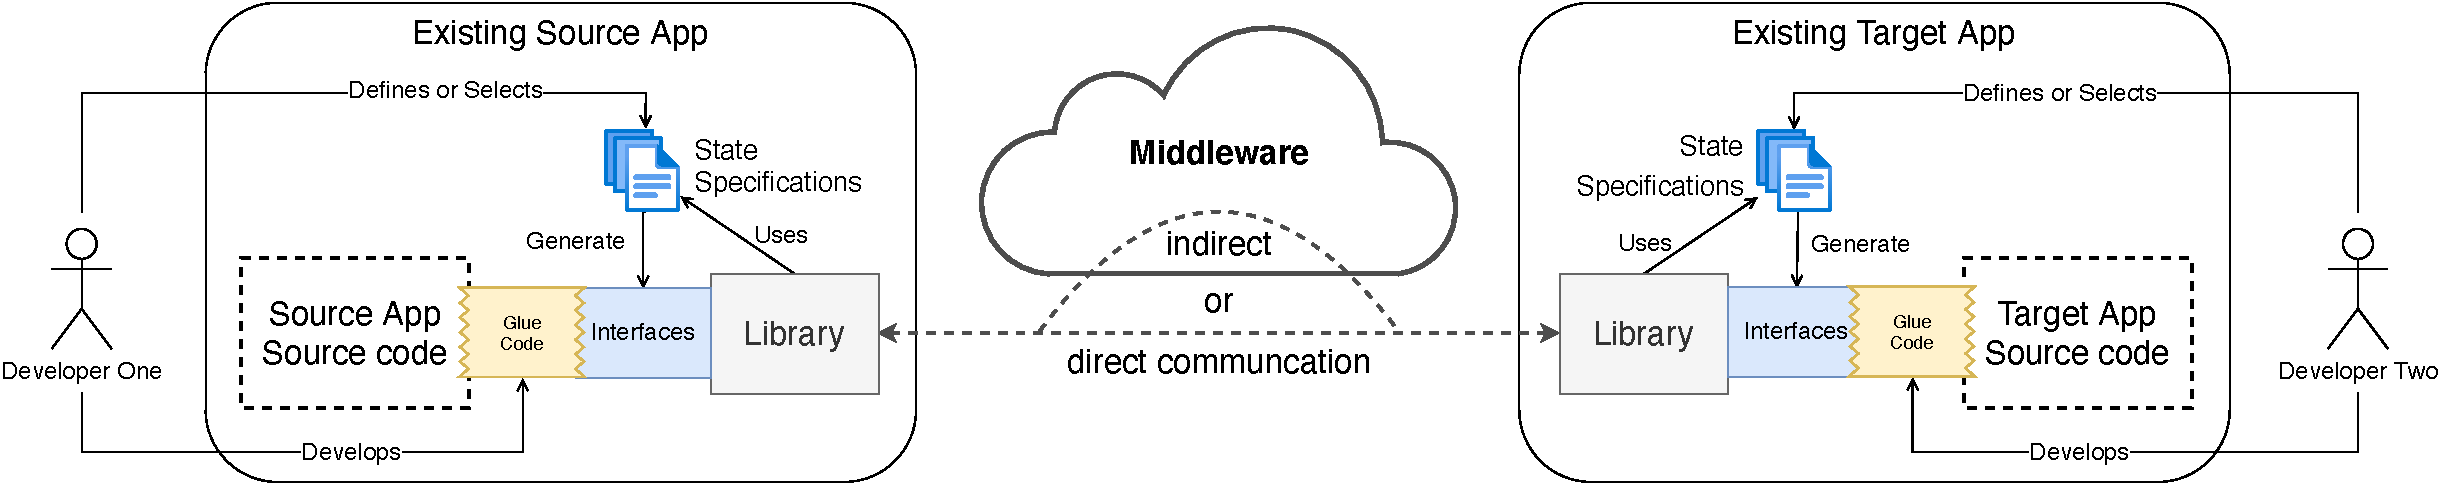
\includegraphics[width=\linewidth]{../figures/solution-overview}
    \centering
    \caption{General overview of the approach}
    \label{fig:solution-overview}
\end{figure}
\FloatBarrier